Рассмотрим работу нашего приложения на примере подготовки такой простой задачи: необходимо для некоторого целого числа $n$ ($2 \leq n \leq 10^{12}$) определить, является ли оно простым, и если является, вывести -1, а в противном случае "--- произвольный его делитель, отличный от единицы и самого числа $n$. Заметим, что в задаче правильный ответ может быть не единственным, поэтому необходимо писать код для чекера. Также мы рассмотрим процесс генерации и валидации тестов, прикрепления авторского решения к задаче и отправки посылки.

На рис.~\ref{screen_problems} отображена вкладка главного окна программы со списком всех созданных задач. Здесь можно добавить или удалить задачу, а также перейти к её редактированию. Как можно видеть, задача <<Prime checking>> уже добавлена.

\begin{figure}[h]
\center{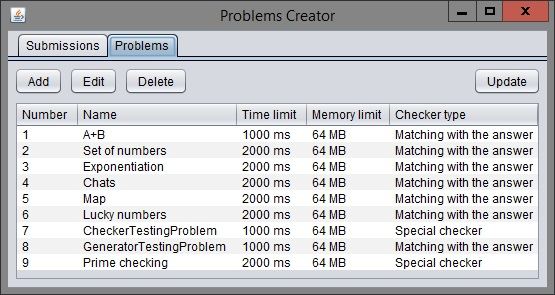
\includegraphics[scale=0.9]{screen_problems}}
\caption{Список созданных задач}
\label{screen_problems}
\end{figure}

Если выбрать задачу и нажать на кнопку <<Edit>>, откроется новое окно с шестью вкладками для редактирования выбранной задачи. На рис.~\ref{screen_problem_param} показана вкладка с основными параметрами задачи: названием, ограничениями по времени и памяти. Также здесь можно загрузить новый файл с условием. Мы выберем ограничения, равные двум секундам и 64-м мегабайтам.

На следующей вкладке (рис.~\ref{screen_tests}) можно посмотреть списки тестов, распределённые по группам, которые можно выбирать в выпадающем списке. Здесь можно добавить или удалить тест, просмотреть входные и выходные данные теста, чтобы изменить их вручную, а также "--- указать количество очков, присуждаемое за один тест из данной группы.

\begin{figure}[h]
\center{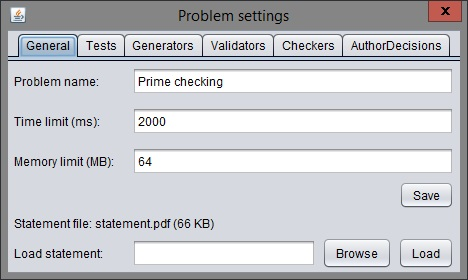
\includegraphics[scale=0.9]{screen_problem_param}}
\caption{Основные параметры задачи}
\label{screen_problem_param}
\end{figure}

\begin{figure}[h]
\center{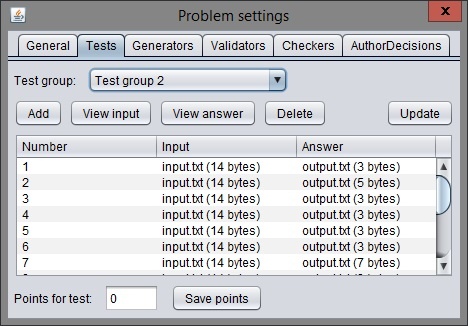
\includegraphics[scale=0.9]{screen_tests}}
\caption{Группа тестов в задаче}
\label{screen_tests}
\end{figure}

\begin{figure}[!ht]
\center{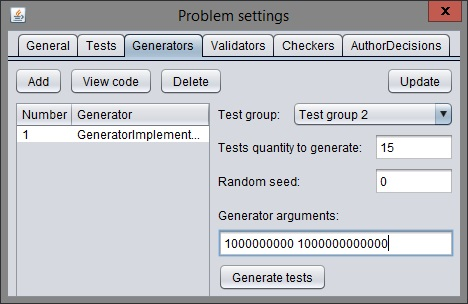
\includegraphics[scale=1.0]{screen_generators}}
\caption{Указание параметров запуска генератора}
\label{screen_generators}
\end{figure}

На вкладке <<Generators>> (рис.~\ref{screen_generators}) можно просмотреть список созданных для этой задачи генераторов, добавить новый (при этом копируется пустой шаблон для генератора) или удалить старый, а также изменить код. На этой же странице можно запускать генератор. Для этого нужно выбрать группу тестов, в которую затем нужно будет сохранить сгенерированные файлы, количество создаваемых тестов, инициализирующее значение для генератора псевдослучайных чисел и строковые параметры генератора, разделённые пробелом.

При нажатии на кнопку <<View code>> открывается окно, отображённое на рис.~\ref{screen_generator_code}. Такое же окно открывается для просмотра и изменения содержимого всех остальных файлов. В данном случае в нём доступен режим редактирования. Для данной задачи достаточно простейшего генератора, принимающего два числовых параметра для определения границ диапазона, в котором должно находиться число $n$ из входных данных, и генерирующего это число.

На рис.~\ref{screen_generator_result} показано окно, которое появится, если мы запустим генератор для создания 15-ти новых тестов для группы <<Tests 2>> с диапазоном для числа $n$ от миллиарда до триллиона. В данном окне отображаются сообщения о ходе процесса генерации тестов, в том числе "--- сколько времени в миллисекундах было потрачено на генерацию каждого теста. Для сохранения сгенерированных тестов в задаче нужно дополнительно нажать на кнопку <<Save>>. Кроме того, можно преждевременно нажать на кнопку <<Interrupt>>, чтобы прервать процесс генерации, если он выполняется слишком долго.

\begin{figure}[!p]
\center{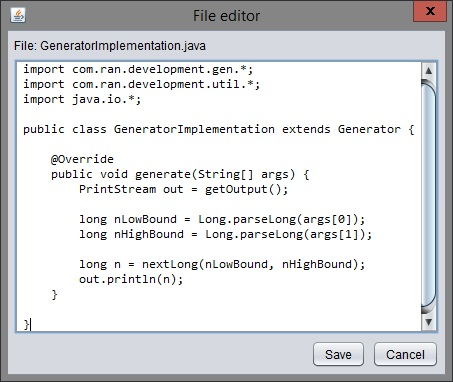
\includegraphics[scale=1.0]{screen_generator_code}}
\caption{Код генератора}
\label{screen_generator_code}
\end{figure}

\begin{figure}[!p]
\center{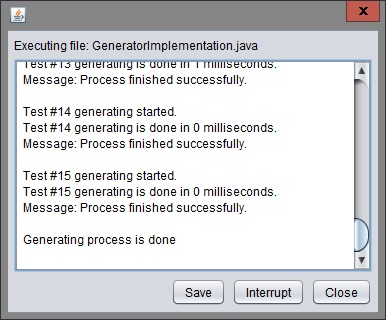
\includegraphics[scale=1.0]{screen_generator_result}}
\caption{Результаты запуска генератора}
\label{screen_generator_result}
\end{figure}

Чтобы просмотреть список прикреплённых к задаче валидаторов, нужно перейти на вкладку <<Validators>>. Здесь так же можно добавить и удалить валидатор, открыть его для редактирования или запустить, указав группу тестов для валидации (или специальный пункт <<All tests>>) и строковые параметры запуска. Данная вкладка отображена на рис.~\ref{screen_validators}. Для данной задачи валидатор также прост: происходит проверка принадлежности числа $n$ диапазону от 2 до $10^{12}$.

На вкладке <<Checkers>> (рис.~\ref{screen_checkers}) можно выбрать тип чекера, используемого при проверке решения данной задачи: либо чекер по умолчанию (<<Matching with the answer>>), либо специальный чекер с написанным для него кодом (<<Special checker>>). Поскольку к одной задаче можно прикрепить только один чекер, здесь не отображается список чекеров. Также отсюда можно открыть окно для редактирования кода чекера и попробовать перекомпилировать его, чтобы удостовериться, что код написан корректно.

\begin{figure}[h]
\center{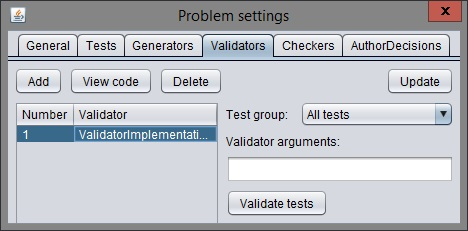
\includegraphics[scale=0.9]{screen_validators}}
\caption{Указание параметров запуска валидатора}
\label{screen_validators}
\end{figure}

\begin{figure}[h]
\center{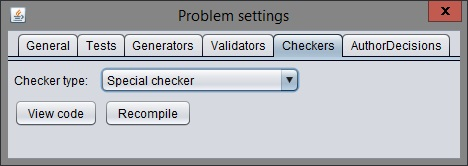
\includegraphics[scale=0.9]{screen_checkers}}
\caption{Указание типа чекера}
\label{screen_checkers}
\end{figure}

Чекер, используемый в данной задаче, выполняет следующие действия. Если участник вывел -1, чекер проверяет, что в ответе жюри тоже находится -1. Если же участник вывел целое число в интервале от 2 до $n$, проверяется, является ли это число множителем $n$.

\begin{figure}[!ht]
\center{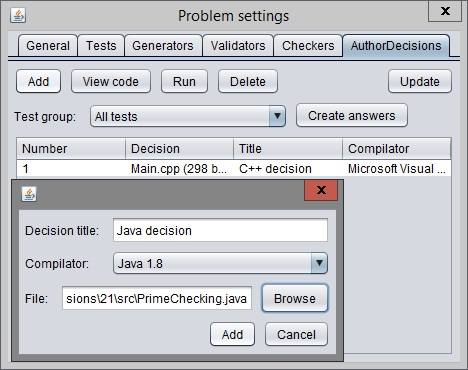
\includegraphics[scale=0.9]{screen_author_decisions}}
\caption{Добавление нового авторского решения}
\label{screen_author_decisions}
\end{figure}

На вкладке <<Author decisions>> можно просмотреть список авторских решений, прикреплённых к задаче (рис.~\ref{screen_author_decisions}). Здесь можно добавить новое решение (при этом отображается маленькое окно для ввода названия решения и выбора компилятора и файла с исходным кодом), удалить решение, открыть его код или запустить, чтобы увидеть вердикт на каждом тесте задачи. Кроме того, кнопка <<Create answers>> запускает генерацию ответов жюри (на каждом тесте из определённой группы, либо на тестах из всех групп, если выбран пункт <<All tests>>).

Главная идея авторского решения состоит в том, чтобы перечислять не все числа от 2 до $n$ для проверки, являются ли они множителем $n$, а только числа от 2 до $\sqrt{n}$, что, очевидно, происходит гораздо быстрее. Решение данной задачи на языке C++ состоит всего из одной функции \texttt{main()}, код которой выглядит следующим образом.

{\small
\begin{verbatim}
long long n;
cin >> n;

int s = (int)ceil(sqrt((double)n));
for (int i = 2; i <= s; i++) {
    if (i != n && n % i == 0) {
        cout << i << endl;
        return 0;
    }
}

cout << -1 << endl;
return 0;
\end{verbatim}
}

\begin{figure}[!b]
\center{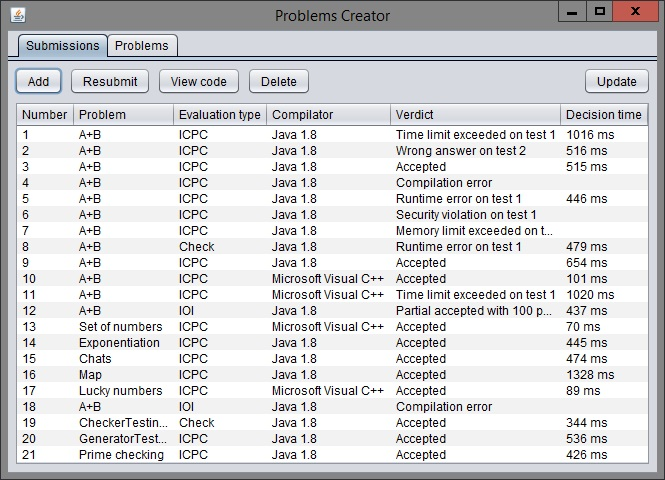
\includegraphics[scale=0.9]{screen_submissions}}
\caption{Список отправленных посылок}
\label{screen_submissions}
\end{figure}

\begin{figure}[!b]
\center{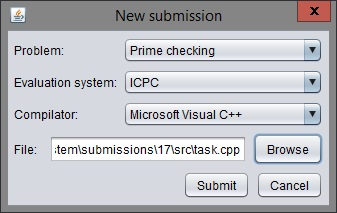
\includegraphics[scale=0.9]{screen_new_submission}}
\caption{Выбор параметров новой посылки}
\label{screen_new_submission}
\end{figure}

Рассмотрим теперь вторую вкладку главного окна приложения (рис.~\ref{screen_submissions}), на которой располагается список всех сохранённых в файловой системе посылок с вердиктами по каждой из них. Здесь можно добавить новую посылку, при этом открывается новое окно, отображённое на рис.~\ref{screen_new_submission}, в котором можно выбрать задачу, компилятор, систему оценивания и файл с исходный кодом. Также на данной вкладке можно удалить посылку, открыть её код для просмотра и перезапустить.

Мы сделаем посылку с решением, написанным на языке Java, но отличающимся от предыдущего рассмотренного решения в способе вывода множителя числа $n$. Если в прошлый раз мы выводили первое найденное число $i$, на которое $n$ делится нацело, то теперь мы будем выводить $n/i$. Ответ всё равно останется правильным, но во многих случаях окажется другим.

Запустим посылку и увидим окно, отображённое на рис.~\ref{screen_submission_results}, где видны вердикт и затраченное время по каждому тесту в задаче. Как можно видеть, такое решение также даёт вердикт <<Accepted>> на всех тестах, что говорит о корректной работе написанного нами чекера.

\begin{figure}[h]
\center{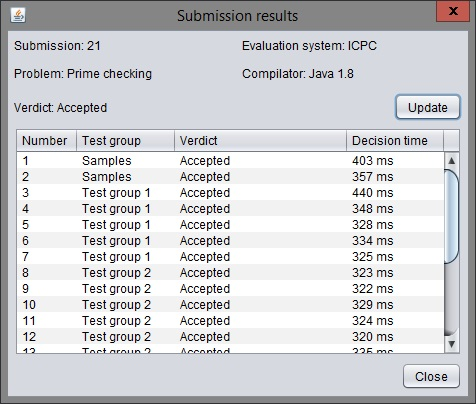
\includegraphics[scale=0.9]{screen_submission_results}}
\caption{Результаты запуска посылки на каждом тесте}
\label{screen_submission_results}
\end{figure}